	
	\chapter{P/NP 基本概念}
	
	\begin{introduction}
		\item $P$,$NP$,$NPC$,$NP-Hard$问题定义
		\item 多项式时间归约
		\item NPC问题概述
		\item P与NP的讨论
	\end{introduction}
	
	\section{引入}
	\begin{table}[!htbp]
		\centering
		\caption{不同算法的复杂度}
		\begin{tabular}{cc}
			\toprule[0.5mm]
			Easy Problem & Hard Problem\\
			(存在多项式复杂度的确定性算法)&(不知道是否存在多项式复杂度的确定性算法)\\
			\midrule[0.4mm]
			最短路问题&最长路径问题\\ \\
			2SAT问题&3SAT问题\\ \\
			2色问题&3色问题\\ 
			\bottomrule
		\end{tabular}
	\end{table}
	
	\section{概念辨析}
	\begin{definition}{$P$类问题}{def1}
	$P$代表$Polynomial$,指存在多项式复杂度的算法的问题。
	\end{definition}

	\begin{definition}{$NP$类问题}{def1}
	$NP$代表$Non-deterministic Polynomial$,指可以在多项式时间内验证一个解,或有一个多项式时间的非确定性算法的问题。
	\end{definition}

	\begin{definition}{$NPC$类问题}{def3}
	$NPC$代表$Non-deterministic Polynomial Complete$,指满足以下两个条件的问题:
	
	(1)它是一个$NP$问题。
	
	(2)所有的$NP$问题都可以在多项式时间归约到它。
	\end{definition}

	\begin{definition}{$NP-Hard$类问题}{def4}
		指满足$NPC$问题的第二条,但不一定要满足第一条的问题。
	\end{definition}
	
	为了更好的阐述这种关系,我们采用它们之间的关系图来对此进行描述,如下图:
	
	\begin{figure}[ht]
		\begin{minipage}[t]{1\linewidth}
			\centering
			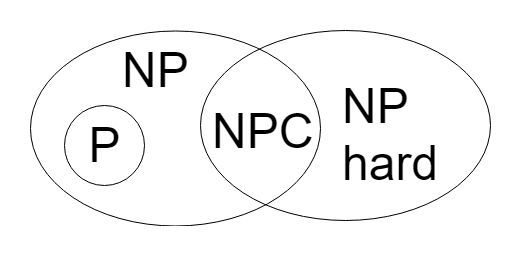
\includegraphics[width=10cm,height=5cm]{image/P_NP1.png}
			\caption{$P$,$NP$,$NPC$,$NPhard$关系图}
		\end{minipage}
	\end{figure}
	
	\section{多项式时间归约}
	\subsection{多项式时间归约的定义与性质}
	在讨论$NPC$问题时我们谈到了多项式时间规约,这里给出了多项式时间规约的定义:
	\begin{definition}{多项式时间规约}{def5}
	多项式时间归约:如果问题$X$和问题$Y$满足以下两条性质,那么问题$X$可以在多项式时间归约到问题$Y$,记作$X\leq_pY$:
		
	(1)问题$X$可以通过多项式时间的基本运算步骤转换为问题。$Y$
	
	(2)问题$X$多项式次调用求解问题Y的算法。
	\end{definition}
	有关多项式时间规约,有以下四条性质:
	\begin{theorem}{多项式规约的四条性质}{}
		(1)如果$X\leq_pY$且$Y$能在多项式时间内求解,则$X$也能在多项式时间内求解。\\
		(2)如果 $X\leq_pY$,且$Y$不能在多项式时间内求解,则$X$也不能在多项式内求解。\\
		(3)如果$X\leq_pY$且$Y\leq_pX$,则$X$,$Y$多项式等价,记为$X\equiv_pY$。若$X$,$Y$中一方能在多项式时间内求解则另一方也能在多项式时间内求解。\\
		(4)归约的传递性:若$Z\leq_pY$且$Y\leq_pX$,则$Z\leq_pX$。
	\end{theorem}

\paragraph*{以下有三点提醒:}

\begin{itemize}
	\item 注意体会上述两个定理中$X$与$Y$的表达顺序;
\end{itemize}
\begin{itemize}
	\item 第二条定理的证明可以采用反证法,假设$X$可以在多项式时间内求解,因为$Y$能够在多项式时间内归约到$X$问题求解,所以$Y$也能在多项式时间内求解,矛盾;
\end{itemize}
\begin{itemize}
	\item $X$的问题比$Y$更“难”。
\end{itemize}

	\subsection{规约问题的举例——染色问题(Graph Coloring)}

\begin{itemize}
	\item $P_1$ (decision version):可用$K$种颜色完成染色
\end{itemize}
\begin{itemize}
	\item $P_2$ (optimal version):最少用$K$种颜色完成染色
\end{itemize}
\begin{itemize}
	\item a)$P_1\leq_pP_2$
	
将$K$值依次从2依次递增,直到$P_1$判定第一个满足的数记为$K_0$,则$K_0$为$P_2$的解,即满足$P_1$的最小的$K$(也就是$K_0$)为$P_2$的解。

过程见下图:
\end{itemize}

	\begin{figure}[ht]
		\begin{minipage}[t]{1\linewidth}
			\centering
			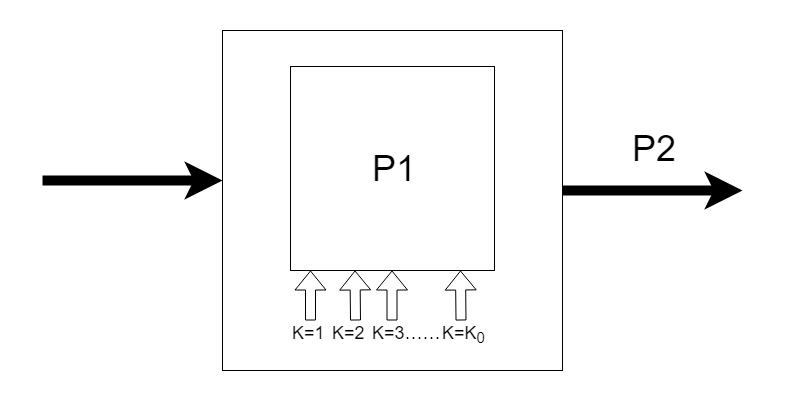
\includegraphics[width=15cm,height=7.5cm]{image/P_NP2.png}
			\caption{$P_1\leq_pP_2$时过程图}
		\end{minipage}
	\end{figure}

\begin{itemize}
	\item b) $P_2\leq_pP_1$
	
	直接利用$P_2$解出$K_0$,判断$K$与$K_0$的关系,若$K\geq K_0$则成立,即可以使用$K_0$种颜色完成染色。
	
过程见下图:
\end{itemize}	

		\begin{figure}[ht]
		\begin{minipage}[t]{1\linewidth}
			\centering
			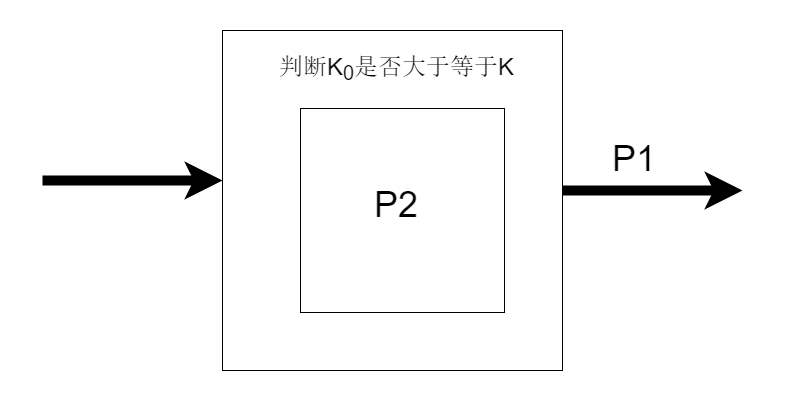
\includegraphics[width=15cm,height=7.5cm]{image/P_NP3.png}
			\caption{$P_2\leq_pP_1$时过程图}
		\end{minipage}
	\end{figure}
	
\newpage
	\section{NPC问题}
	\subsection{NPC概述}

\begin{itemize}
	\item $NPC$问题的证明思路
	
要证明一个问题是$NPC$问题,先证明它是一个$NP$问题,然后再证明一个已知的$NPC$问题能在多项式时间归约到它。
\end{itemize}

\begin{itemize}
	\item $NPC$问题与$NP$问题之间的关系
\end{itemize}

\begin{itemize}
	\item $NPC$问题是比普通的$NP$问题更复杂一点的问题,如果找到一个$NPC$的多项式复杂度算法,也就能够通过降阶的方式将这个算法改造成解决任意一个确定的$NP$问题的多项式复杂度算法。意味着存在一个通用的万能算法,能够解决所有$NP$问题,这样只要找到一个$NPC$的多项式算法也就证明了$P=NP$。
\end{itemize}	


\begin{itemize}
	\item $NPC$问题举例
\end{itemize}	

	\begin{table}[!htbp]
		\centering
		\caption{NPC问题举例}
		\begin{tabular}{p{100pt}p{200pt}}
			\toprule[0.5mm]
			问题 & 描述\\
			\midrule[0.4mm]
			布尔可满足性问题&给定一个布尔方程,判断是否存在一组布尔变量的真值指派使整个方程为真的问题\\ \\
			最小顶点覆盖问题&给定图$G=(V,E)$和数$k$,判定是否存在包含大小至多为$k$的顶点覆盖。\\ \\
			集合覆盖问题&给定全集$U$,以及一个包含$n$个集合且这$n$集合的并集为全集的集合$S$。集合覆盖问题要找到的一个最小的子集$S$,使得他们的并集等于全集\\ \\
			哈密尔顿回路&给定图$G$,判定其是否经过图中每个顶点且仅一次的回路。\\
			\bottomrule
		\end{tabular}
	\end{table}
\section{关于P与NP的讨论 (P=NP?)}

\begin{itemize}
	\item$P\subseteq NP$
	
如果一个问题能够在多项式时间求解,那么这个问题则一定可以在多项式时间内被验证
\end{itemize}
\begin{itemize}
	\item $P$是否能够等于$NP$,即等价于一个问题的结果如果能够用多项式复杂度的算法来验证,那么是否存在多项式算法来得出这个结果。现在没人能够证明这一点。
\end{itemize}
\begin{itemize}
	\item 证明的关键点在于能否找到一个$NPC$的多项式算法。但$NPC$问题目前没有多项式算法,只能用穷举法逐个检验得到答案。所以现在科学家们普遍认为$P\neq NP$
\end{itemize}
\begin{itemize}
	\item假设证明了$P= NP$,目前的加密技术就会没有前途,因为目前的加密技术是将一个整数分解为几个因数的乘积,正是因数分解过程烦琐,才保证了信息的安全。
\end{itemize}
	
以下列出了$P= NP$与$P\neq NP$两种情况的情况如下图所示:
	
	\begin{figure}[!htbp]
		\begin{minipage}[t]{1\linewidth}
			\centering
			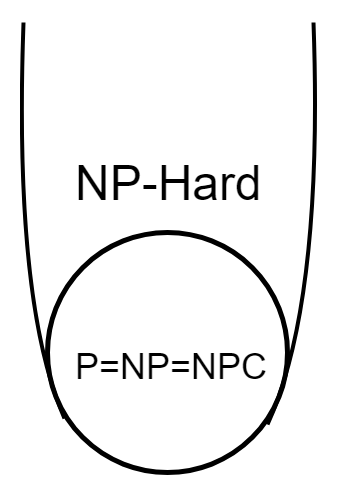
\includegraphics[width=4cm,height=6cm]{image/P_NP4.png}
			\caption{$P= NP$时关系图图}
		\end{minipage}
	\end{figure}

		\begin{figure}[!htbp]
		\begin{minipage}[t]{1\linewidth}
			\centering
			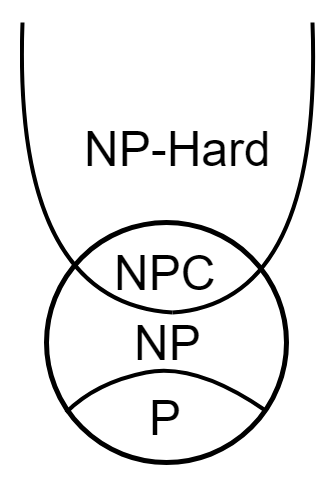
\includegraphics[width=4cm,height=6cm]{image/P_NP5.png}
			\caption{$P\neq NP$时关系图}
		\end{minipage}
	\end{figure}
	
